\chapter{Related work}
In 2007, the notion of bandwidth as a currency was introduced.
In 2009, the first Bitcoins were mined\cite{Blockchain.info-bcs}.
These events can be seen as the first steps in reputation or currency systems.
Currencies have more strict rules to work than a reputation system.
In this chapter we will discuss related work on tamper-proof interaction histories in currency or reputation systems.
The block chain used in Bitcoin is explained extensively,
because there is much similairity between MultiChain.
Understanding these concepts in the block chain helps understanding MultiChain.
The differences between the block chain and MultiChain will be explained in section \ref{sect:scalable-reciprocity}.
Bartercast is the current implemented reputation system used by Tribler that will be replaced by MultiChain.
Several other related systems are finally briefly discussed.

\section{Block chain}
\label{sect:bitcoin}
Bitcoin is a digital currency that uses a global, full transaction history
to keep track of transactions made between nodes.
It is called a global, full transaction history,
because the transaction history is shared between every peer and contains every transaction.
The transaction history is a datastructure called the block chain.

The block chain imposes limits on Bitcoin in several ways.
These limitations on Bitcoin can be seen as the initial motivation for our work.
How Bitcoin uses the block chain technology will be introduced first.
In the following sections the limitations imposed by the block chain will be explained.

We will only introduce how Bitcoins uses the block chain and why it does so.
The best starting point for a full explanation of Bitcoins
is the original paper by Nakamoto\cite{Nakamoto-bitcoin}.
Further information on Bitcoin can be found on the Bitcoin website\cite{Bitcoin.org-site}.

\subsection{Transfer of ownership of a bitcoin}
The core of the Bitcoin protocol is the block chain.
The block chain contains transactions of bitcoins.
We will first describe how the transactions are build up
and later how they are part of the block chain.

A transaction consists of three parts.
The first part is the public key of the new owner of the bitcoin.
The hash of the whole, previous transaction and the public key of the new owner is concatenated.
This concatenation is hashed and this hash is the second part of the transaction.
The final part is the signature by the current owner of this new hash.
Inclusion of the hash of the previous transaction chains a transaction to the previous transaction.

The previous transaction is a transaction of the same bitcoin.
The ownership of the bitcoin by the current owner can be verified
by verifying the whole chain of ownership of the bitcoin.
A transaction is usually shortend to Tx in Bitcoin related work and is used in images in this report.
In Figure \ref{fig:bt-transaction-chain} a diagram can be seen of how transactions are chained.

\begin{figure}
	\centerline{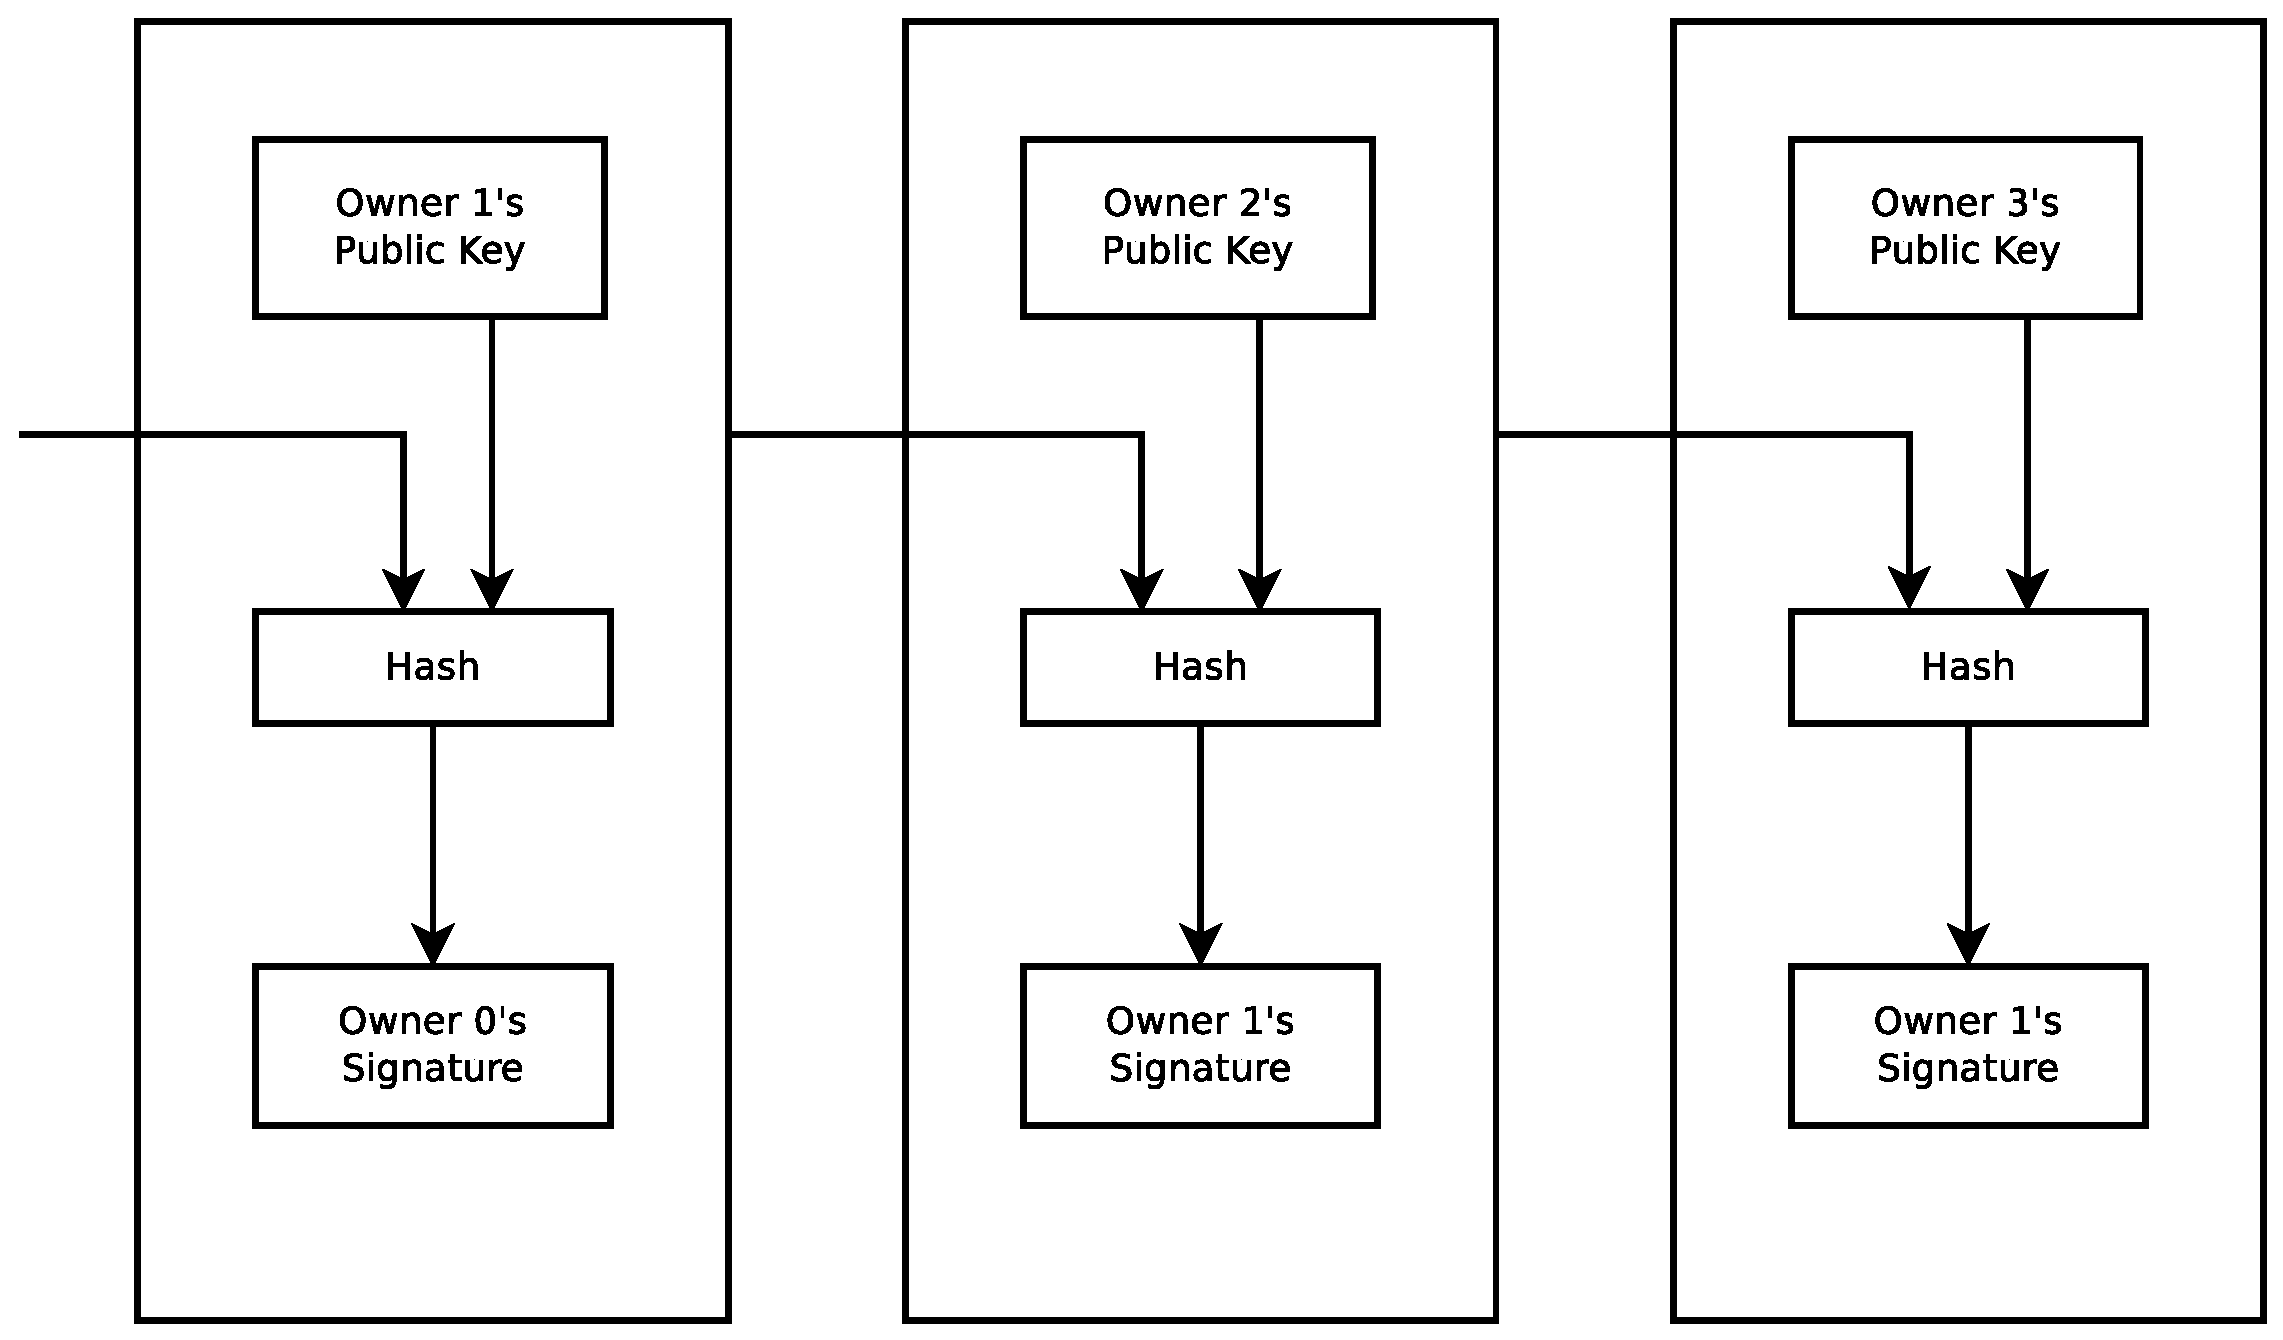
\includegraphics[scale=0.3]{relatedWork/figs/transactions.eps}}
	\caption{Transfer of ownership of bitcoin in a transaction chain.}
	\label{fig:bt-transaction-chain}
\end{figure}

\subsection{Block chain}
Multiple transactions are aggregrated into a single block.
Every block contains the hash of the previous block.
This creates the block chain.
Transaction chains span across several blocks inside the block chain.
A diagram can be seen in Figure \ref{fig:bt-block-chain} of the block chain.

\begin{figure}
        \centerline{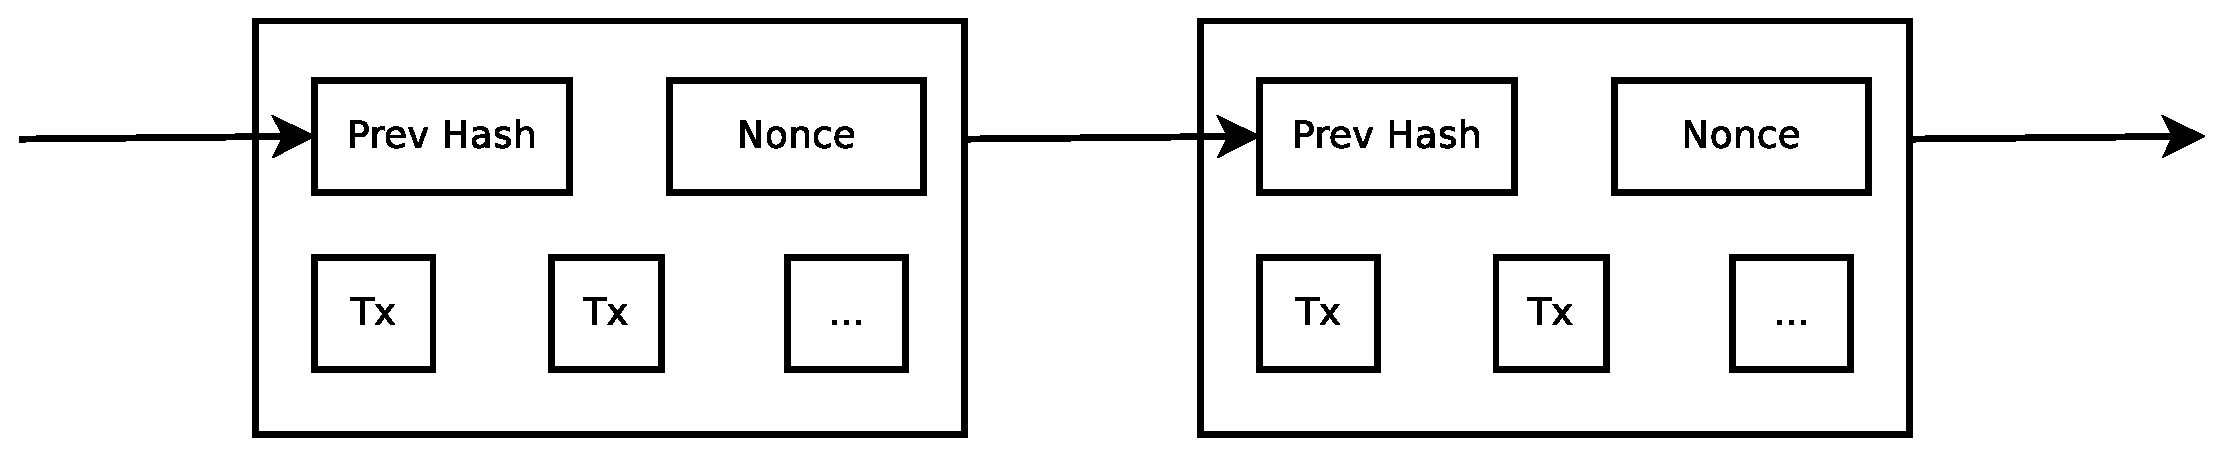
\includegraphics[scale=0.3]{relatedWork/figs/blocks.eps}}
        \caption{Block chain}
        \label{fig:bt-block-chain}
\end{figure}

These blocks in the block chain are created by nodes in the network, so called miners.
A miner receives transactions from other nodes in the Bitcoin network.
An attacker could malicously transmit transactions to double spend a bitcoin he owns or does not have.
So every transaction is verified on arrival at a node.
Any transaction that double spends a bitcoin is simply dropped by the node.
No penalty is awarded to the malicous attacker.

The transactions are received in a non deterministic way induced by network characteristics.
The non deterministic nature causes blocks to differ from miner to miner.
The order of transactions has to be agreed upon by the network to eliminate this inconsistency.

Bitcoin uses election to pick the next block based upon a Proof-Of-Work system.
A nonce is added to every block.
This nonce is just a number that can be varied,
but is only sound if the hash of the whole block starts with a certain number of zeros.
Miners have to find the correct nonce for their block and this is a proof of work.

However, miners can still find a valid nonce at approximately the same time
and notify parts of the network of their newly found block.
This also leaves the network in an inconsisted state.
Multiple versions of the next block attached to the previous block can be seen as branches.

To solve this inconsistency, Bitcoin nodes save both branches and continue using the longest branch.
At some point one branch will become predominant in the network.
More nodes will dedicate compute power to extend this branch and the growth rate will increase for this branch.
The faster growth rate will ensure that the branch will be adopted by the network as a whole.
The smaller branch is abandoned and the blocks are orphaned.

The amount of zeros, needed in the hash of the transaction,
is adjusted to compensate for the fluctuating speed of the network to be able to find nonces.
The speed of the network is called the hash rate and is the amount of hashes calculated per second.
The amount of zeros balances the probability of branches occuring
and the time before a new block is found,
which in turn is how fast transactions are processed.
The amount of zeros can be seen as the difficulty\cite{bitcoin-difficulty} of finding the a block.
More zeros decreases the likelyhood a nonce will be valid.
The estimated hash rate over time can be seen in Figure \ref{fig:hash-speed}\cite{Blockchain.info-hashspeed},
and the difficulty in Figure \ref{fig:hash-difficulty}\cite{Blockchain.info-difficulty}.

\begin{figure}[h]
        \centerline{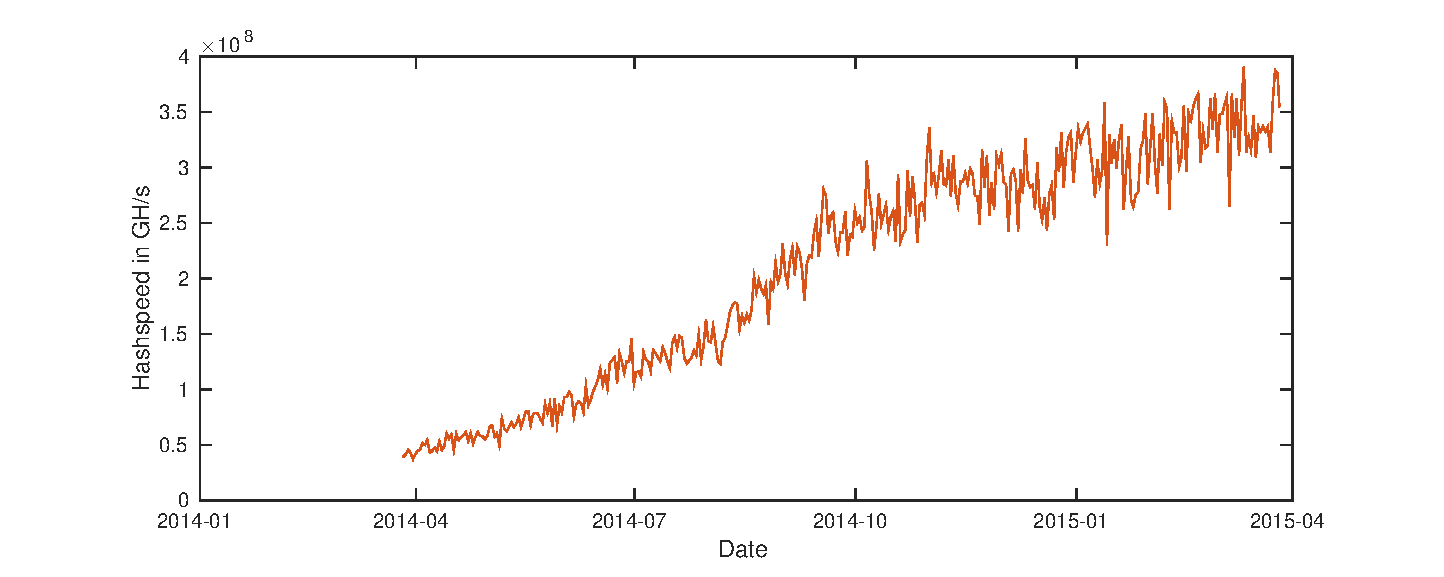
\includegraphics[scale=0.5]{relatedWork/figs/hashspeed/hashspeed.eps}}
        \caption{Estimated amount of hashes per second.}
	\label{fig:hash-speed}
\end{figure}

\begin{figure}
        \centerline{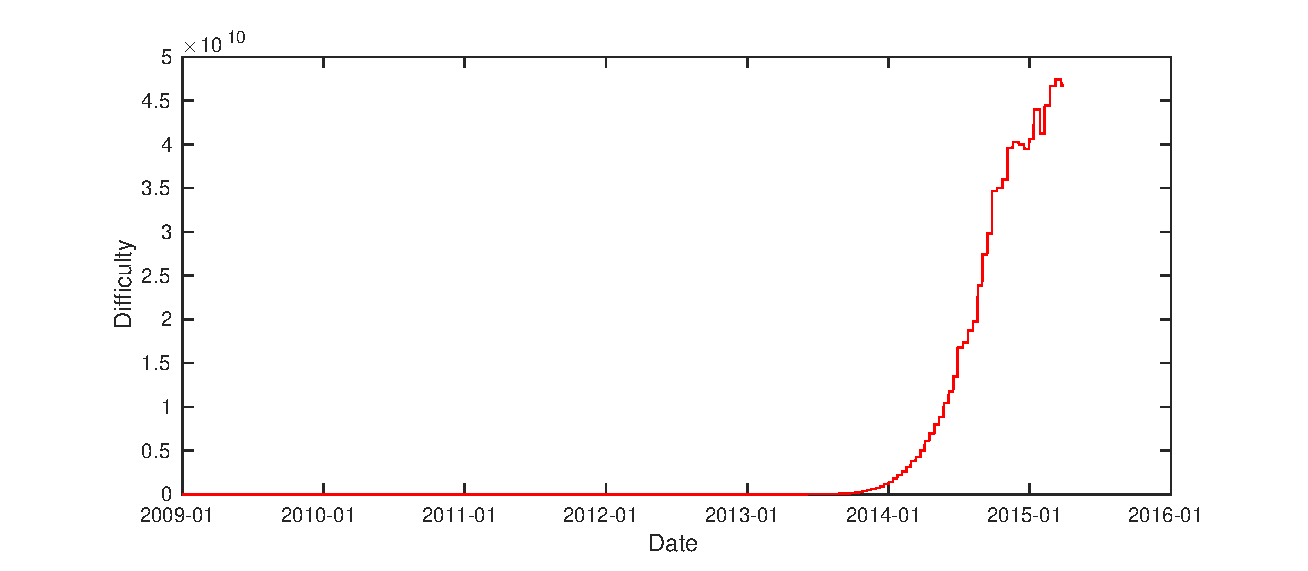
\includegraphics[scale=0.5]{relatedWork/figs/difficulty/difficulty.eps}}
	\caption{The difficulty of finding blocks.}
	\label{fig:hash-difficulty}
\end{figure}

Another possible attack to double spend a bitcoin is by sending a transaction to one part of the network,
but to the other part of the network a transaction with a different receipient.
It is possible that both transactions will be introduced into the block chain, but in different branches by two independend miners.
Eventually one branch will win and the attack is averted.

The behaviour just described causes that a transaction can never be confirmed with full certainty.
The possibility always exists that another branch over takes the current longest branch.
This makes the network vulnerable if the total compute power is owned by a malicous attacker is more than the total compute power of the honest nodes,
even if the attacker only has control of 51\% of the compute power.
In the end the current branch can be overtaken by a new branch started by the attacker.
This new branch allows the whole transaction history to be rewritten by the attacker.

\subsection{Limitations}
In this section we will discuss the several limitations of Bitcoins
that originate from the use of the block chain.

\subsubsection{Size}
\label{bitcoin-limit-size}
To be able to prevent double spending and enable rightful spending by the owner,
the node verifying a transaction needs to be aware of the full history of a bitcoin.
This results in that a node needs the entire block chain.

The block chain is a data structure ever increasing in size.
No block or data contained in that block is removed.
The block chain has been growing since its inception in 2009.
The size and growth can be seen in Figure \ref{fig:bc-size}.

\begin{figure}
        \centerline{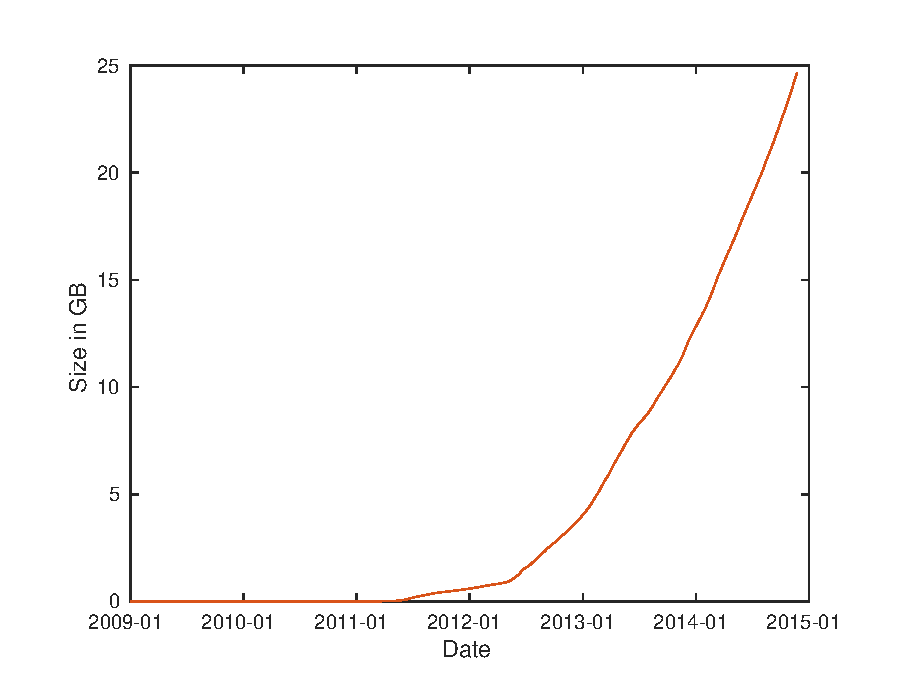
\includegraphics[scale=0.6]{relatedWork/figs/blockchainsize/blockchainsize.eps}}
        \caption{The size of the block chain.\cite{Blockchain.info-bcs}}
	\label{fig:bc-size}
\end{figure}

The size of the block chain at time of writing already prevents less powerful devices, like smartphones,
to operate on the block chain.
This problem is only going to become bigger with the continued creation of transactions
and at a faster pace due to increased adoption of Bitcoin.
The growth of the size of the block chain has already outpaced the growth of the power of a smartphone
and will also be relatively larger compared to other types of hardware.

This problem was already identified by Nakamoto in his original paper on Bitcoin.
The paper proposes Simplified Payment Verification (SPV).
In SPV mode a node only downloads the block headers of the longest chain.
If a transaction is to be verified, it requests from the network the specific transaction
along with a Merkle tree linking it to a block in the chain.
The Merkle tree can be used to verify that the transaction was included into the block chain.
This allows to calculate with some confidence that the transaction was accepted.

SVP only gives reasonable confidence and is not as secure as running a full node.
Trust has to be placed in the nodes that send the block headers and Merkle Trees.
Secondly, a transaction that is recorded in a more recent block is less difficult to tamper with
than a transaction deep down in the block chain.
This is only an acceptable solution for clients willing to accept more risk due to having a less secure system.
Therefor it is not a solution for the problem for every one.

\subsubsection{Amount of transactions}
The usability of a digital currency is in part determined by the time it takes to process a transaction
and how many transactions can be processed in a certain time scale.
The amount of transactions that can be handled by Bitcoins are determined by two factors:
\begin{itemize}
\item Block size
\item Block creation time
\end{itemize}

The block size is currently capped at a fixed maximum size.
A block can be smaller, but cannot exceed the maximum size.
The current blocksize limit is 1MB.
A block has a fixed part and the rest is filled up by transactions picked by the miner.
A transaction can vary in length.
The number of transactions that can be fitted inside a block is limited by the maximum size.

This maximum size has no clear documentation of why it was picked as such.
There are several implications of raising the size, aswell as lowering.
Increasing the block size will increase the number of transactions that can be processed.
But the increased block size will increase propogation time of the block in the network.
A longer propogation time will in turn result in a higher orphane rate of the miner.

Large clusters of hash power owned by a single miner or mine cluster can be placed closer together
reducing propogation time for this miner.
This will benefit this single miner in reducing his orphaned rate
and will increase the chance of his block being adopted.
This will make the network as a whole more susptible to attack by a single powerful miner
and will reduce the power of other miners.

The difficulty of finding a new block roughly regulates how fast new blocks are created.
The difficulty is set according to the hash rate of the whole network to equal roughly a new block every 10 minutes.
If the time of finding a new block is decreased,
then more blocks are generated and obviously more transactions can be fitted inside these blocks.
The reverse is true if the time is increased.
But the time between blocks is a balance between the orphan rate of blocks
and how fast transactions are committed to the block chain.

These two factors currently result in a theoretical limit of 7 transactions per second\cite{bitcoin-transactions}.
This can be calculated by dividing the maximum blocksize with the minimal size of a transaction.
The performance of Bitcoin can be changed by changing the settings of these two factors.
This limits the global usage of Bitcoins.
In comparison, Visanet, that handles transactions under Visa,
is able to process 54.000 transactions per second\cite{visa-transactions}.
To be a real replacement of the current traditional currencies
a higher number of transactions per second have to be achieved by a digital currency.
There are at time of writing several competing proposals to increase the block size\cite{garzik-blocksize}\cite{andresen-blocksize}.



\section{BarterCast}
\label{sect:bartercast}
BarterCast is the system used by Tribler to incentivise good behaviour by keeping track of reputations
\cite{pouwelse-buddycast}\cite{meulpolder-bartercast}\cite{meulpolder-bartercast-paper}\cite{dumitrescu-tribler}.
It is fully decentralized, in contrast to previous reputation systems in a peer-to-peer network.
Private BitTorrent communities, for example, depend on central servers to track reputation\cite{meulpolder-bartercast}.
BarterCast was not designed with the aim to be fully resistant to malicious nodes
that want to falsify their reputations.
The initial version has been first deployed in June 2006
and subsequently has been improved.
BarterCast will be briefly explained as well as its vulnerabilities.

\subsection{Epidemic protocol}
At the base of BarterCast is BuddyCast.
BuddyCast is an epidemic protocol stack and BarterCast is part as a protocol of this stack.
A overview of the BuddyCast stack can be seen in Figure \ref{fig:buddycast-stack}
and a more thorough introduction can be found in the report on BuddyCast\cite{pouwelse-buddycast}.

\begin{figure}
	\centerline{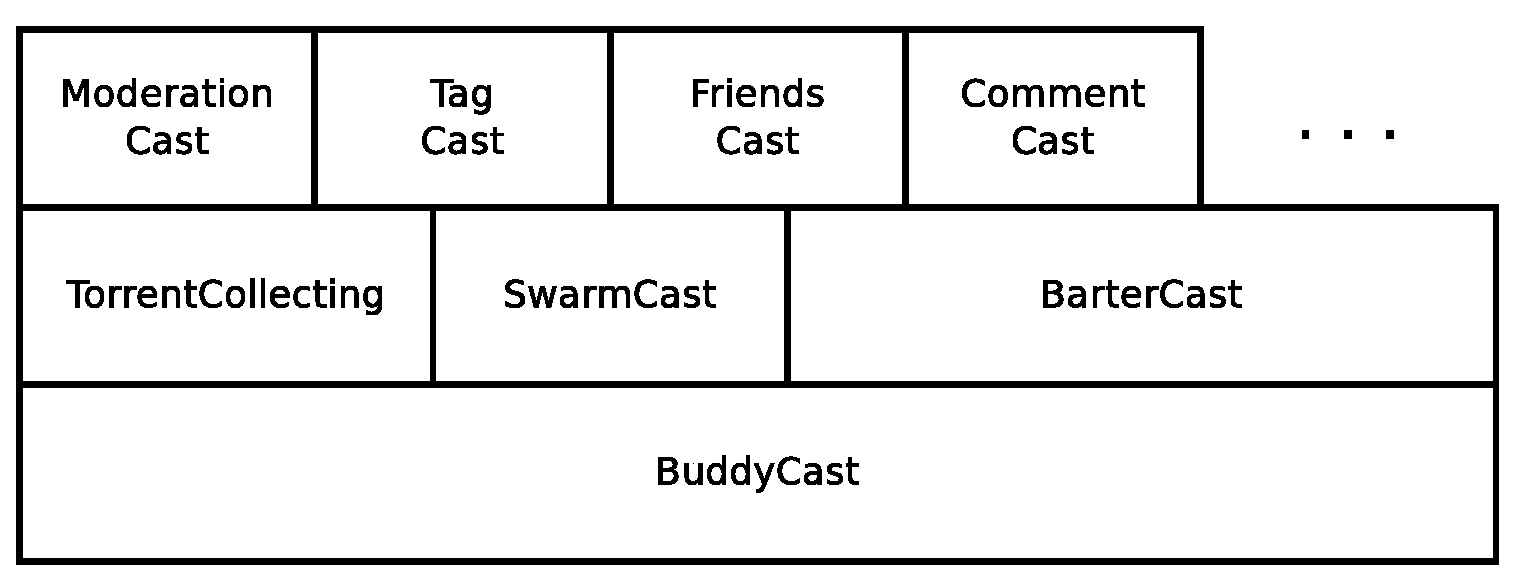
\includegraphics[scale=0.3]{relatedWork/figs/buddycast-stack.eps}}
	\caption{BuddyCast stack overview\cite{pouwelse-buddycast}.}
	\label{fig:buddycast-stack}
\end{figure}

An epidemic protocol works in a very simple way relying on a receive-and-forward primitive.
Information is exchanged and forwarded between peers.
This is called gossiping.
BarterCasts gossips on the donation of upload bandwidth
and the consumption of download bandwidth by other peers.

BuddyCasts spreads information of other peers with initial messages.
This is done every 15 seconds, but a peer is only contacted every 4 hours to avoid contacting too often.
These messages contain a prefered content list, a list of peers with similair prefered content
and a list of random peers.
For each peer a public key, IP adress, port number and last seen timestamp is provided.
The peers with a similair preference are called taste buddies.
A format of the these messages can be seen in Figure \ref{fig:buddycast-format}.

\begin{figure}
	\centerline{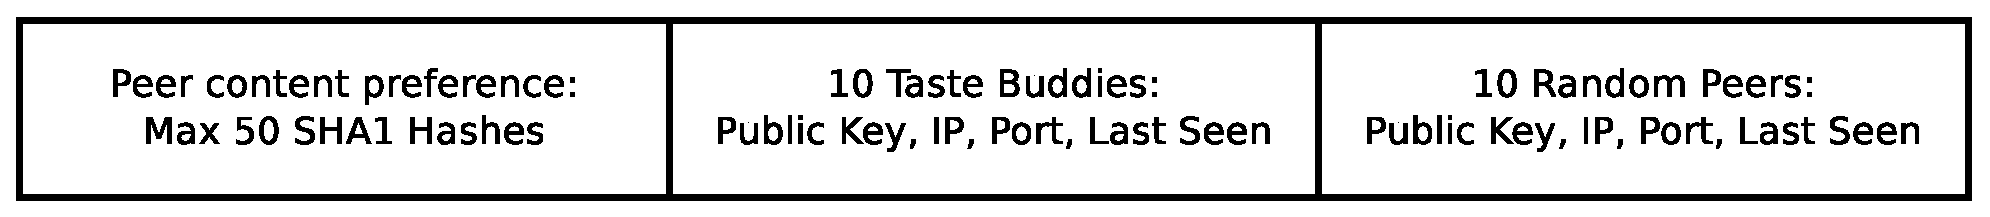
\includegraphics[scale=0.3]{relatedWork/figs/buddycast-format.eps}}
	\caption{Format of initial messages in BuddyCast\cite{pouwelse-buddycast}.}
	\label{fig:buddycast-format}
\end{figure}

BuddyCasts uses several techniques to improve the peer selection efficiency.
Peer selection efficiency is the percentage of successfully delivered outgoing messages to peers.
This metric measures how well BuddyCasts selects peers on availablity and connectablity.
These are important because they determine how well BuddyCasts is able to handle with peer failure and exit.
Sending messages to an unavailable peer is a complete waste of resources.

The most obvious improvement that has been made is not to forward any offline peers.
BuddyCast maintains a live overlay
and continuously verify the online status of 10 random peers and 10 taste buddies.
The random peers are updated to ensure they are in fact random peers.

Peers can detect their own connectivity issues.
While they are able to connect outbound,
no incoming connections can be excepted.
These peers can improve the peer selection efficiency
by broadcasting that they are having connectivity problems
and instructing others to not gossip their identity.

Each peer collects information on how much other peers have downloaded and uploaded.
This information is signed and a barter record is created.
These barter records are forwarded to 10 peers.
A peer has a chance to be random peer or a taste buddy.
The records are forwarded by attaching them to BuddyCast messages.

The aggregrated information contains information about direct interactions with other peers,
but also information about interactions between other peers gossiped.
The information can be visualised using BarterBowser.
A screenshot can be seen in Figure \ref{fig:barterbrowser}.
The center contains the local peer.
Every circle contains peers for a certain degree.
The first circle from the centre contains peers that the local peer has direct interactions with.
The second circle contains peers that peers from the first circle has direct interactions with and so forth.
The figure shows how BarterCast accumulates data through other peers.

\begin{figure}
	\centerline{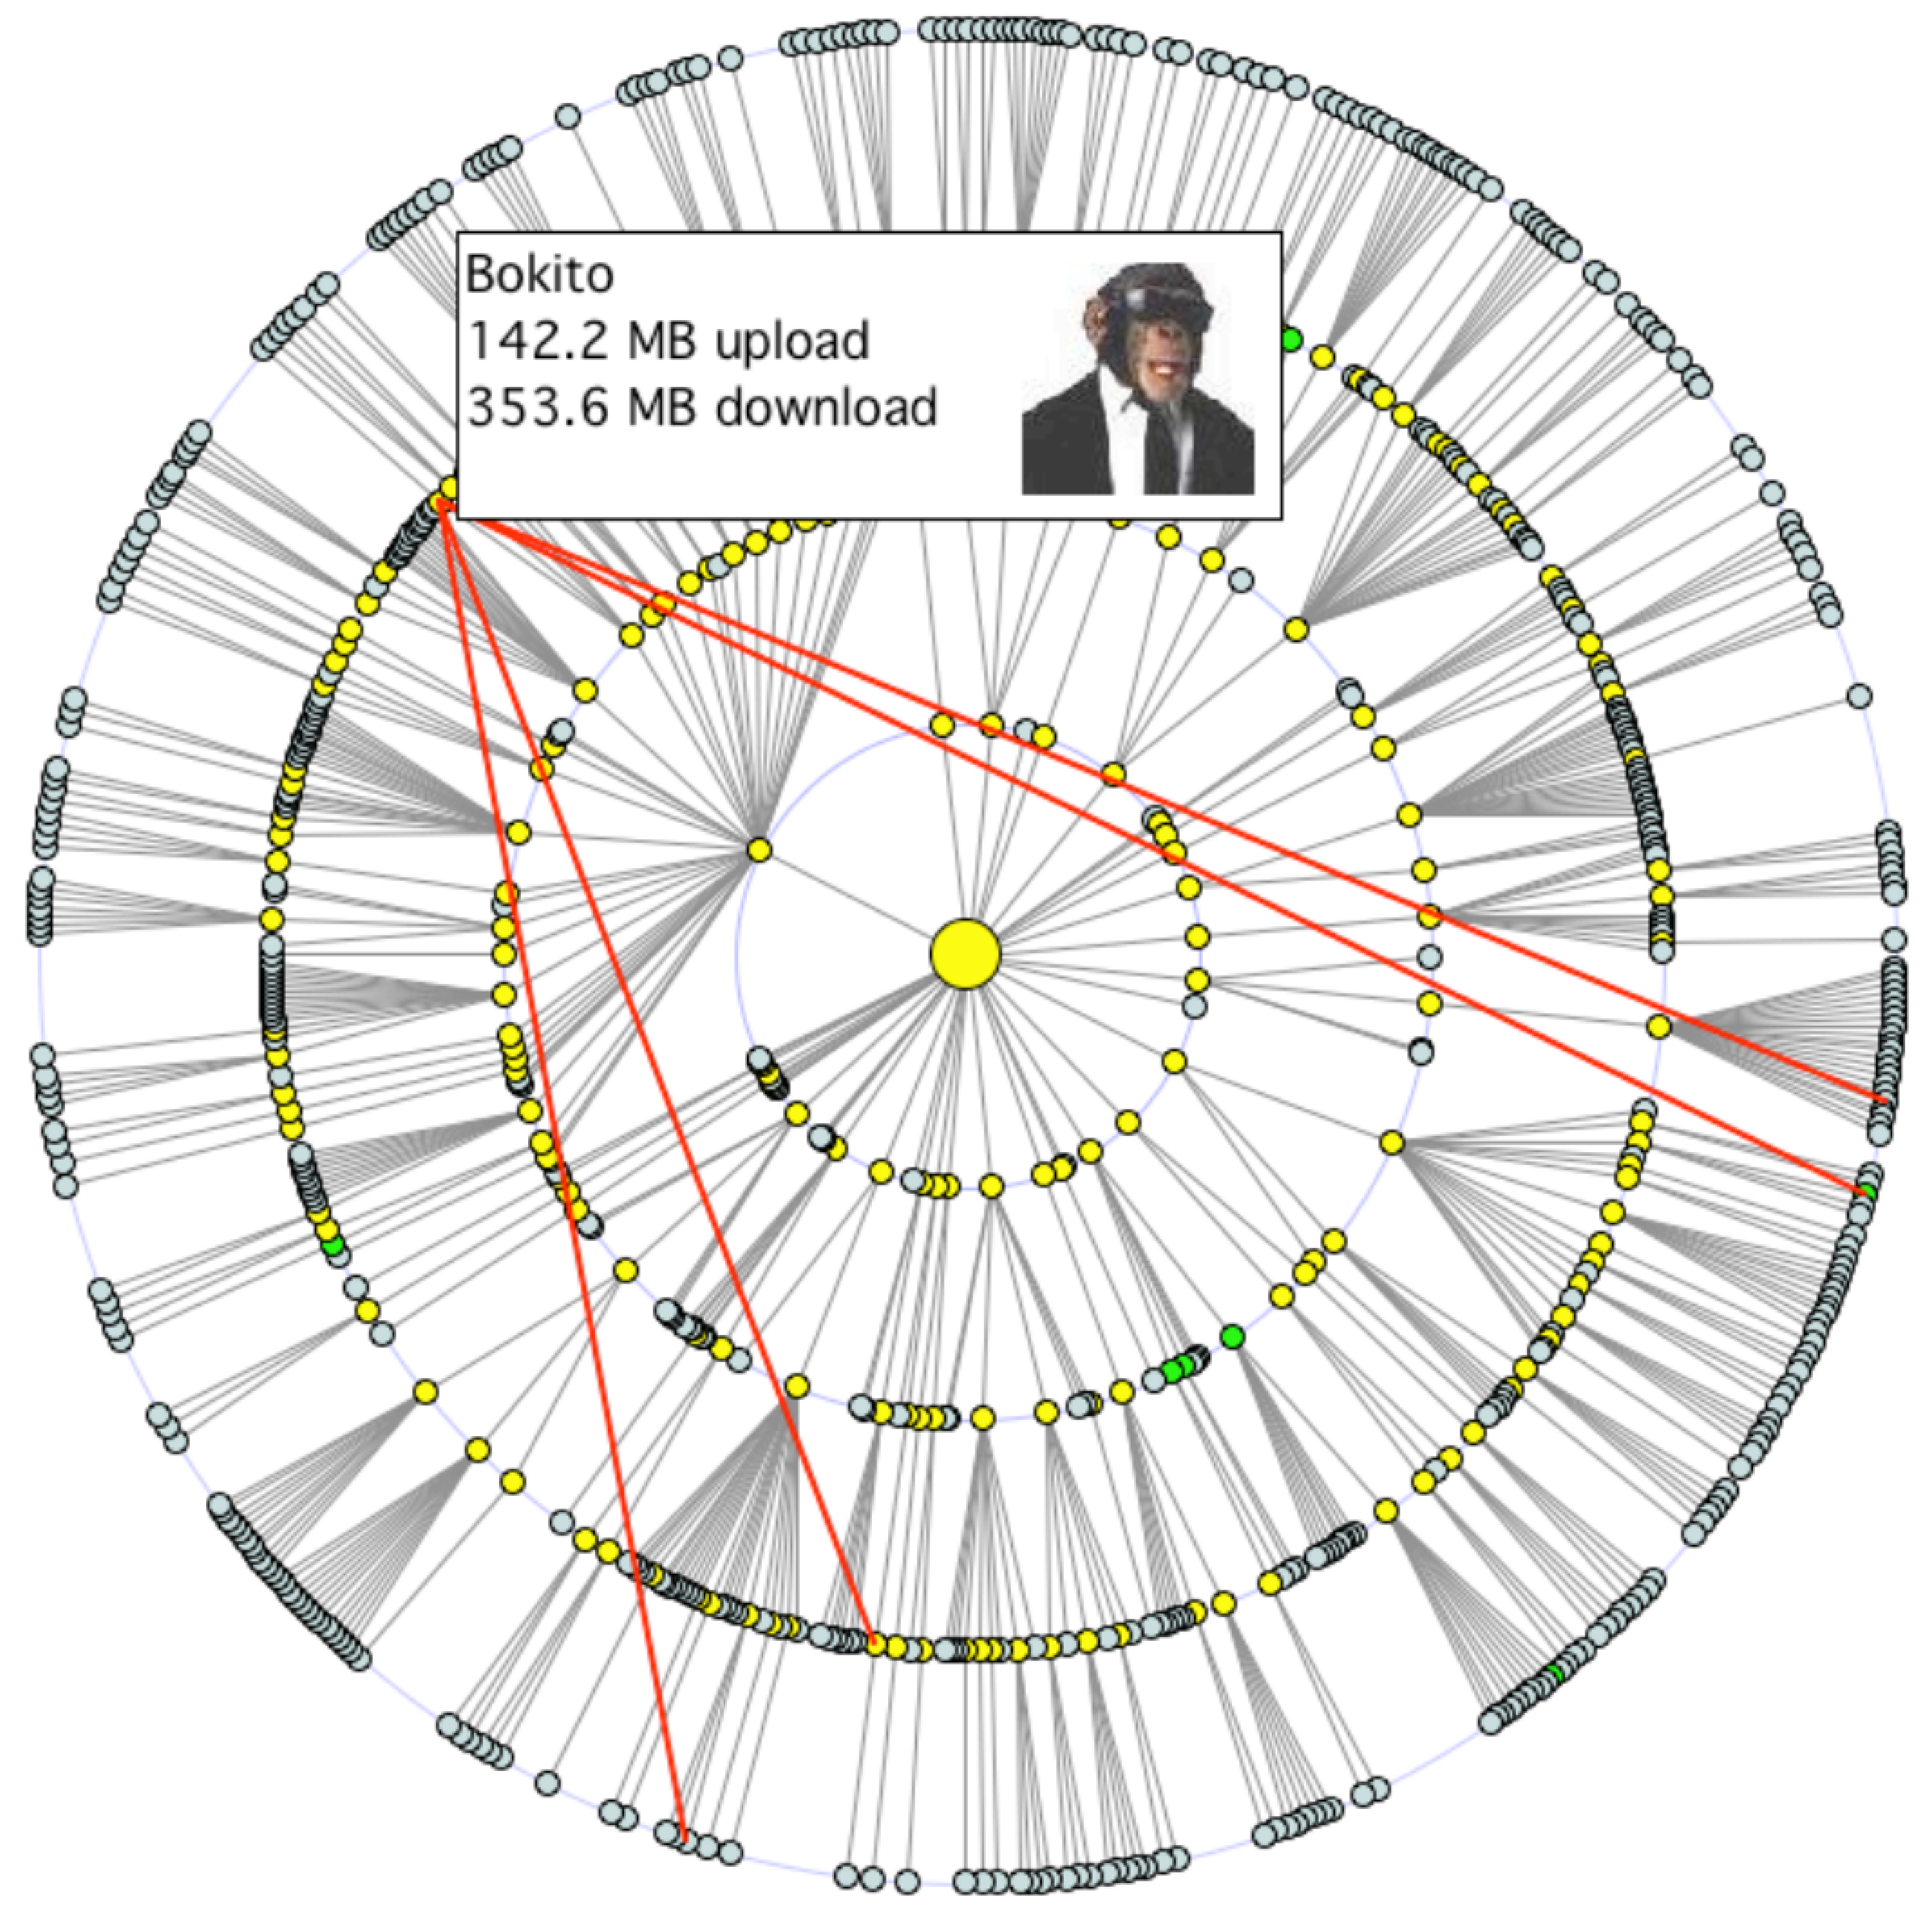
\includegraphics[width=0.8\textwidth]{relatedWork/figs/barterBrowser.eps}}
	\caption{A screenshot of BarterBrowser in 2008\cite{pouwelse-buddycast}.}
	\label{fig:barterbrowser}
\end{figure}

The information can be used to in conjunction with the maxflow algorithm
to create a reputation metric\cite{meulpolder-bartercast-paper}.
The reputation metric measures how well or how poorly a peer has helped the network.
The calculation takes into account that the difference between 0 and 100 MB is more significant
then between 1000 MB and 1100 MB.

The calculation is done without relying on a third party.
No authority verifies the validity of the received information.
Also there is no insurance that the information is complete.

Improvements have been done to improve the performance of BarterCast.
A bloom filter algorithm is implemented to decrease the amount of duplicate barter records
being sent to peers already having those records\cite{logiotatidis-splash}.
Bloom filters can be used to quickly determine with some certainty
if a database contains records in limited space\cite{broder-bloomfilter}.
The bloom filter protocol works in the following way:
\begin{enumerate}
    \item Peer $A$ creates a specific Bloom filter for peer $B$.
    \item Peer $A$ sends the Bloom filter to peer $B$.
    \item Peer $B$ checks every record in its database using the Bloom filter.
    \item Peer $B$ sends any missing record to peer $A$.
\end{enumerate}
The created bloom filters only contain relevant entries that have not yet been synchronized to peer $B$.
BarterCasts knows which entries are relevant by keeping track of the last synchronization point
and only using new barter records since that point.

\subsection{Limitation}
The proposal of this thesis is to implement a new reputation system for Tribler,
so obviously Bartercast is lacking.
The main problem with Bartercast, and why it needs to be replaced with a new system is
that the reputation is self reported.
Barter records are not signed by any one else.
So Barter records can be created by any malicious node without a limit.
There is no way to verify these records and enforce truthfulness.
Finally, there is no way to punish malicious nodes and therefore they are free to lie.





\section{Other related work}
The topic of reputation system is currently a subject of research for other projects as well
and show the struggle to build a working reputation system.
There are two projects worth to briefly mention, because of similairity to the Tribler project.
These projects are not so thoroughly explained as the block chain
as they were not used as a starting point in designing MultiChain.

The Tor project is working on a implementation of a reputation system in an effort to incentivize collaboration\cite{dingledine-torincentive}.
There are currently multiple proposals: PAR\cite{androulaki-torincentive}, BRAIDS\cite{jansen-braid}, LIRA\cite{jansen-lira}, TEARS \cite{jansen-torincentive}, TorCoin\cite{ghosh-torincentive}, and XPAY\cite{chen-torincentive}.
The amount of proposals demonstrate the complexity of creating a reputation system in an anonymous system.

The InterPlanetary File System \(IPFS\) is a peer-to-peer distributed file system with similairities to the Tribler project.
IPFS uses an incentivized block exchange to improve collaboration\cite{benet-ipfs}.